\documentclass[]{jocg}

\usepackage{amsmath,amsfonts}
\usepackage{amsthm}

\usepackage[utf8]{inputenc}
\usepackage[english]{babel}
\usepackage{mathtools}
\usepackage[mathlines]{lineno}
\usepackage[]{graphicx}
\usepackage{algorithm}
\usepackage[noend]{algpseudocode}
\linenumbers

\usepackage[
  backend=biber,
  style=alphabetic,
  sorting=ynt
]{biblatex}
\addbibresource{main.bib}


\newcommand{\RR}{\mathbb{R}}
\newcommand{\PP}{\mathcal{P}}
\newcommand{\EE}{\mathcal{E}}
\newcommand{\set}[1]{\{#1\}}
\newcommand{\norm}[1]{\|#1\|}
\newcommand{\abs}[1]{|#1|}
\newcommand{\chordarc}{s_{\abs{\partial~\cdot~}}}
\DeclareMathOperator{\diam}{\mathrm{diam}}
\DeclareMathOperator{\conv}{\mathcal{}}



\newtheorem{proposition}{Proposition}[section]

\theoremstyle{definition}
\newtheorem{definition}[proposition]{Definition}

\theoremstyle{remark}
\newtheorem{remark}[proposition]{Remark}


\title{%
  \MakeUppercase{Measuring polygonal niceness}%
  \thanks{%
    This paper comprises the completion of the final project for AMS 545
    ``Computational Geometry''.
  }
}

\author{%
  Sharmila~Duppala%
  \thanks{%
    \affil{Department of Computer Science}, 
    \email{sduppala@cs.stonybrook.edu}%
  }\, and
  David~Kraemer.%
  \thanks{%
    \affil{Department of Applied Mathematics},
    \email{david.kraemer@stonybrook.edu}%
  }
}

\begin{document}

\maketitle

\begin{abstract}
\end{abstract}

\tableofcontents

\section{Introduction}

\begin{enumerate}
  \item Paragraph introducing general problem
  \item Paragraph on applications to gerrymandering problems.
  \item Paragraph explaining the limitations of this application. (Perhaps this
    should be in the discussion?)
  \item Paragraph outlining the paper.
\end{enumerate}

\section{Theoretical background}

The area of a subset $S \subseteq \RR^2$ of the plane is denoted by
$\lambda(S)$. We will denote the boundary of $S$ by $\partial S$. For two points
$x,y \in \RR^2$, the closed line segment with endpoints in $x$ and $y$ is
denoted $[x,y]$. For $p \in [1, \infty]$, we define the $p$-ball as $B_{p}(x,
\varepsilon) = \set{y \in \RR^2 : \norm{x-y}_p \leq \varepsilon}$ and we will
only be interested in the closed case. Unless otherwise stated, we shall operate
in the Euclidean world with $p = 2$. Throughout we shall assume that $P
\subseteq \RR^2$ is a simple bounded closed polygon. The class of such polygons
is given by $\PP$. Its perimeter is denoted by $\abs{\partial P}$.

\subsection{The $\alpha$-fatness score}

One approach to measuring the relative ``fatness'' of a polygon seeks to
identify regions of the shape which behave highly unlike balls.

\begin{definition}
  The $\alpha$-fatness score of a polygon $P$ is given by
  \begin{equation*}
    \alpha(P) = \inf\set{\frac{\lambda[P \cap B(x,
    \varepsilon)]}{\lambda[B(x,\varepsilon)]} : \varepsilon > 0, x \in P}
  \end{equation*}
  where we impose that the ball $B(x,\varepsilon)$
  does not contain $P$. 
  \label{def:alpha}
\end{definition}

The constraint that $P \not\subseteq B(x,\varepsilon)$ ensures definiteness:
otherwise, let $\varepsilon \to \infty$ and the ratio $\frac{\lambda[P \cap B(x,
\varepsilon)]}{\lambda[B(x, \varepsilon)]}$ always approaches $0$. An intuition
for $\alpha(P)$ emerges from considering how it behaves on balls.

\begin{proposition}
  For any $P$, $\alpha(P) \leq \frac{1}{4}$, and if $P = B(x_0, r)$
  then we have equality.
  \label{prop:alpha}
\end{proposition}

\begin{proof}
  To show that $\alpha(P) \leq \frac{1}{4}$, it suffices to show only for convex
  $P$, because $P \subseteq \conv(P)$ implies $\lambda[P \cap B(x, \varepsilon)]
  \leq \lambda[\conv(P) \cap B(x, \varepsilon)]$. Let $d = \diam (P)$ and fix
  $x,y \in \partial P$ such that $\abs{[x,y]} = d$. Assume without loss of
  generality that $x$ lies above $y$, and consider the ball $B(x, d)$. Then $P$
  does not meet the upper disk of $B(x,d)$, for otherwise we could choose $z \in
  P$ in the upper disk of $B(x,d)$ which forms a chord of $P$ longer than $d$.
  A similar argument shows that $P$ cannot occupy more than half of the lower
  disk of $B(x,d)$. Hence
  \begin{equation*}
    \alpha(P) \leq \frac{\lambda[P \cap B(x,d)]}{\lambda[B(x,d)]} \leq
    \frac{1}{4},
  \end{equation*}
  as needed.

  The fact that $\alpha(B(x_0, r)) = \frac{1}{4}$ relies on a neat
  result \cite{10.2307/30044198} that shows that the $L_p$
  ellipsoid $\EE$ with radii $a, b$ has area
  \begin{equation*}
    \lambda(\EE) = a b \cdot 4
    \frac{\Gamma(1+\frac{1}{p})^2}{\Gamma(1+\frac{n}{p})}.
  \end{equation*}
  In our case, $\alpha(B(x_0, r))$ is achieved at a ball on a ``corner'' point
  with radius $2r$.
\end{proof}

Hence, the $\alpha$-score is greater for polygons which exhibit ``niceness''
characteristics. It is not affected tremendously by local nonconvexity in $P$ so
long as $P$ ``snugly fits'' into a ball shape, which is a global property.

\subsection{The chord-$f$ score}

A different class of ``fatness'' measures arises through partitioning $P$ into
two (interior disjoint) polygons $P = P' \cup P''$ via chords. A chord is a pair
$x,y \in \partial P$ such that the segment $[x,y]$ is contained in the interior
of $P$ except at the endpoints $x$ and $y$. Such a chord defines a partition of
$P = P' \cup P''$ by orientation, so that $\partial P'$ is the arc from $x$ to
$y$ together with $[x,y]$ and that $\partial P''$ is the arc from $y$ to $x$
together with $[x,y]$.

\begin{definition}
  Let $f : \mathcal{P} \to \RR$. For a given $P \in \mathcal{P}$, its
  \emph{chord-$f$ score} is given by
  \begin{equation*}
    s_f (P) = \inf \set{\max(f(P'), f(P'')) : x, y \in \partial P}
  \end{equation*}
  where the chord $[x,y]$ partitions $P = P' \cup P''$.
  \label{def:chord-f}
\end{definition}

The intuition for $f$ is some global measure of ``cost'' associated with respect
to $P$. For example, if $f(P) = \abs{\partial P}$, then $s_f$ identifies the
partition (or limiting sequence of partitions) which minimizes the maximum
subpolygon perimeter. Indeed, measures such as perimeter or area are the typical
choices of $f$, but any suitable property of $P$  may be employed. 

The chord-$f$ score can be understood relatively simply in the context of a
minimax game. Max, given a polygon with a chord partitioning it, always chooses
the subpolygon associated with a greater $f$ (i.e., the worst cost of the
partition). Min, who plays first, tries to find a chord with the least-bad worst
cost with respect to $f$.

The member of this class of scores under this present investigation is
$\chordarc$, the so-called \emph{chord-arc} score. It is important to note that
the length of the chord $[x,y]$ which partitions $P$ is included in the
estimation of $\chordarc$. One implication of this is that the chord-arc score
need not be bounded above by $\frac{\abs{\partial P}}{2}$.  We have several
facts about $\chordarc$ which develop further intuition for the score.
\begin{proposition}
  \begin{enumerate}
    \item Let $R$ be a rectangle with height $h$ and length $\ell$. Assume that
      $h \leq \ell$. Then $\chordarc(R) = 2h + \ell$.
    \item Let $P$ be convex with perimeter $\abs{\partial P} = w$. Then
      $\chordarc(P) \leq \frac{w}{2} + \diam (P)$.
    \item Let $C$ be a circle with ``perimeter'' $2\pi r$. Then $\chordarc(C) =
      (\pi + 2)r$.
  \end{enumerate}
  \label{rem:chordarc}
\end{proposition}

\begin{proof}
  \begin{enumerate}
    \item That the optimal partition bisects $R$ is readily apparent,
      for this minimizes the maximum perimeter length of either sub-rectangle.
      A case analysis confirms that the preferred strategy for Min is to choose
      a chord along the smaller dimension (i.e., $h$) to bisect $R$, and in this
      case the maximum arc length is $2h + 2\left( \frac{\ell}{2} \right) = 2h +
      \ell$, as needed.
    \item For $P$ convex, a perimeter-bisecting chord, whose length is at most
      $\diam(P)$, always exists. 
    \item This follows from part 2 by noticing that the length of \emph{any}
      perimeter-bisecting chord is $\diam(C) = 2r$. \qedhere
  \end{enumerate}
\end{proof}

\section{Overview of empirical design}

In principal of computing the $\alpha$ and chord-$f$ scores relies on sweeping
the continuum of points of $P$ and evaluating the aforementioned measurements.
To estimate this process in practice, we employ the following discretizing
scheme. Let $P$ be determined by the vertices $[v_1, \dots, v_n]$ given in
counterclockwise order. Then, given $\delta > 0$, loop through the vertices of
$P$, checking if $\norm{v_{i+1} - v_i} > \delta$. In the case where this holds,
we insert $v_i' = \frac{v_i + v_{i+1}}{2}$ after $v_i$ into the polygon and
resume the loop. This ensures that for any two adjacent vertices $v_{i}$ and
$v_{i+1}$ in the representation of $P$ we have $\norm{v_{i+1} - v_i} \leq
\delta$. As $\delta \to 0$ this estimates $\partial P$ more exactly. All
computations are done with respect to the $L_{\infty}$ norm. The implementation
of this procedure is given in Algorithm \ref{alg:delta}.

%% Pseudocode for the delta refinement

\begin{algorithm}[h]
  \begin{algorithmic}[0]
    \Procedure{RefineBy}{$P,\delta$}
    \State{$P = [v_1, v_2, v_3, \dots, v_n]$};
    \State{$v = v_1$}
    \While {$\textit{next}(v) \ne v_1$}
    \If {$\norm{\textit{next}(v) - v}_2 > \delta$}
      \State{\textrm{Insert $\textit{midpoint}(v, \textit{next}(v))$ into $P$
      after $v$}} 
      \Comment{Now $\textit{next}(v)$ is the midpoint}
      \EndIf
      \EndWhile
      \EndProcedure
    \end{algorithmic}
    \label{alg:delta}
\end{algorithm}

Given a $\delta$-refined polygon $P$, the computation of $\alpha(P)$ is
relatively straightforward, with the simplification that points $x$ on which the
ratio is computed lie on $\partial P$. The computation steps through $[v_1,
\dots, v_n]$ and for each $v_i$ the radius $\varepsilon$ of the
minimum-enclosing $\infty$-ball centered at $v_i$ is computed. Then for
$\varepsilon_k = \frac{k}{100} \varepsilon$, $k = 1, \dots, 100$, the ratio 
\begin{equation*}
  \frac{\lambda[P \cap B_{\infty}(v_i, \varepsilon_k)]}{B_{\infty}(v_i,
  \varepsilon_k)}
\end{equation*}
is computed and the smallest such ratio is kept. The minimum over all $v_i$ is
given as $\alpha(P)$. The implementation of the $\alpha$ score is given in
Algorithm \ref{alg:alpha}. 

%% Pseudocode for the alpha score

\begin{algorithm}[h]
  \begin{algorithmic}[0]
    \Function{$\alpha$Score}{$P$}
    \State{$P = [v_1, v_2, v_3, \dots, v_n]$};
    \State{$\textrm{min} = \infty$}
    \For {$v \in P$}
    \State{$\varepsilon = \textrm{radius of minimum enclosing ball of $P$ at
    $v$}$}
    \For {$k = 1, 2, \dots, 100$} \Comment{$100$ is arbitrary}
    \State{$\varepsilon_k = \frac{k}{100} \varepsilon$}
    \State{$\textrm{area} = \frac{\lambda[P \cap B_{\infty}(v, \varepsilon_k)]}{B_{\infty}(v, \varepsilon_k)}$}
    \If {$\textrm{min} > \textrm{area}$}
      \State{$\textrm{min} = \textrm{area}$}
      \EndIf
      \EndFor
      \EndFor
      \State{\Return{\textrm{min}}}
      \EndFunction
    \end{algorithmic}
  \label{alg:alpha}
\end{algorithm}

Similarly, given a $\delta$-refined polygon $P$, the chord-$f$ score is computed
by sweeping all possible chords of $P$. For each point $v_i, v_j \in \partial P$
with $i < j$, if $[v_i, v_j]$ is indeed a valid chord of $P$, the partition $P =
P' \cup P''$ is computed and the maximum of $f(P')$ and $f(P'')$ is kept. The
minimum such value is given as $s_f(P)$. The implementation of the chord-$f$
score is given in Algorithm \ref{alg:chordf}.

%% Pseudocode for the chord f score

\begin{algorithm}[h]
\begin{algorithmic}[0]
  \Function{ChordScore}{P,f}
  \State{$P = [v_1, v_2, v_3, \dots, v_n]$};
  \For {$v \in P$}
  \For {$w \in [\textit{next}(v), \dots, v_n]$}
  \If {$[v,w]$ is a chord of $P$}
    \State{Partition $P = P' \cup P''$ by $[v,w]$}
    \State{$\textrm{submax} = \textit{max}(f(P'), f(P''))$}
    \If {$\textrm{min} > \textrm{submax}$}
      \State{$\textrm{min} = \textrm{submax}$}
      \EndIf
    \EndIf
  \EndFor
  \EndFor
  \State{\Return{\textrm{min}}}
  \EndFunction
\end{algorithmic}
\label{alg:chordf}
\end{algorithm}

All of these algorithms are implemented in CGAL \cite{cgal:eb-18a} with the
extensive use of the 2D Polygon library \cite{cgal:gw-p2-18a}.


\section{Empirical results}


We evaluate our measurements on randomly generated polygons with vertices in the
unit square $[0,1] \times [0,1]$. We consider collections of such polygons of
10, 50, and 100 vertices. In Figure \ref{fig:delta}, we measure the effect of
sweeping $\delta$ between $0.05$ and $1$ on the resulting measurements. Figure
\ref{fig:alph-inft-10} shows a comparison of $\alpha$-fatness and
${\chordarc}_{\infty}$ scores for polygons on 10 vertices. Figure
\ref{fig:alph-one-50} shows a similar comparison of $\alpha$-fatness and
${\chordarc}_{1}$ scores for polygons on 50 vertices.

\begin{figure}[t]
  \centering
  %\includegraphics{<+file+>}
  \caption{Effect of sweeping $\delta$ on measurements}
  \label{fig:delta}
\end{figure}<++>

\begin{figure}[t]
  \centering
  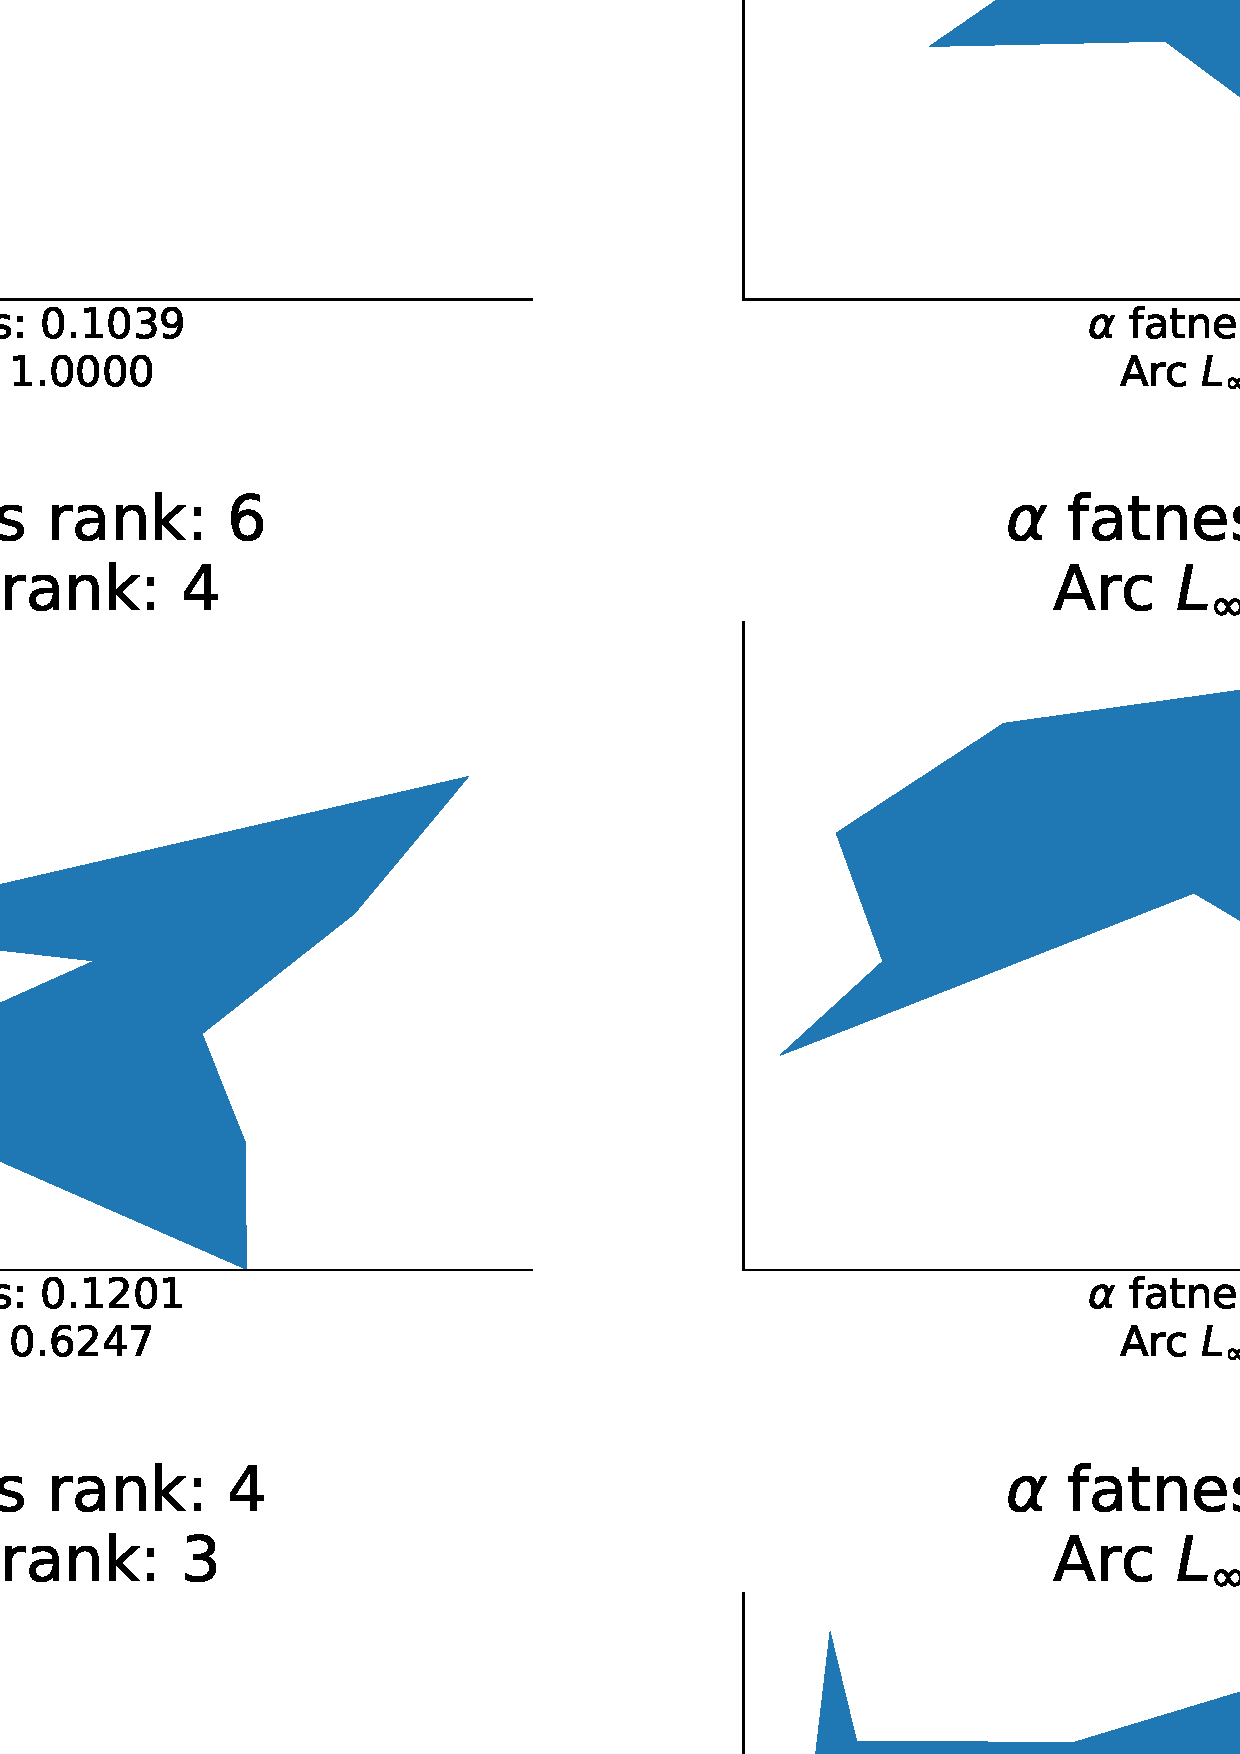
\includegraphics[height=0.8\textheight]{../plots/u_10_alpha_score_chord_arc_infinity_vertices_0-05_delta_ranking.jpg}
  \caption{$\alpha$ scores and ${\chordarc}_{\infty}$ scores for randomly
  generated polygons on 10 vertices.}
  \label{fig:alph-inft-10}
\end{figure}

\begin{figure}[t]
  \centering
  \includegraphics[height=0.8\textheight]{../plots/u_50_alpha_score_chord_arc_one_vertices_0-05_delta_ranking.jpg}
  \caption{$\alpha$ scores and ${\chordarc}_{\infty}$ scores for randomly
  generated polygons on 50 vertices.}
  \label{fig:alph-inft-10}
\end{figure}


\begin{enumerate}
  \item Show how changing $\delta$ affects scores.
  \item Compare scores (by ranking) on random polygons.
  \item Compare scores (by ranking) on U.S. state boundary data.
\end{enumerate}

\section{Discussion}

\begin{enumerate}
  \item Comment on the results.
  \item Talk about applications to Gerrymandering.
\end{enumerate}

\medskip

\printbibliography[heading=bibintoc]

\end{document}
